\documentclass[aspectratio=169]{beamer}
\usetheme{Singapore}

\title{Sample Presentation}
\author{Your Name}
\date{\today}


\usepackage[style=abnt]{biblatex}
\addbibresource{bibliografia.bib}

\usepackage[dvipsnames]{xcolor}




\begin{document}

\frame{\titlepage}

\begin{frame}
\frametitle{Sumário}
\tableofcontents
\end{frame}

\section{Introdução}

\begin{frame}
    \frametitle{Por que cidades existem?}

    \begin{columns}
        \column{0.5\textwidth}
        \begin{itemize}
            \item Cidades são movidas por ``newcomers'' \cite{bauman2003city}
        \end{itemize}

        \column{0.5\textwidth}
        Right column content.
    \end{columns}
\end{frame}

\begin{frame}
    \frametitle{Motivação econômica}
\end{frame}


\begin{frame}
    \frametitle{O problema do custo social}
\end{frame}

\begin{frame}
    \frametitle{Regulação em São Paulo}
\end{frame}

\begin{frame}
    \frametitle{O problema}
\end{frame}

\section{Teoria}

\begin{frame}
    \frametitle{Construção do modelo econômico}
\end{frame}

\begin{frame}
    \frametitle{Resultados principais}
\end{frame}

\begin{frame}
    \frametitle{Implicações em policy}
\end{frame}


\section{Dados}

\begin{frame}
    \frametitle{Dados do Censo}
    \begin{columns}
        \column{.4\textwidth}
        \begin{figure}
            \centering
            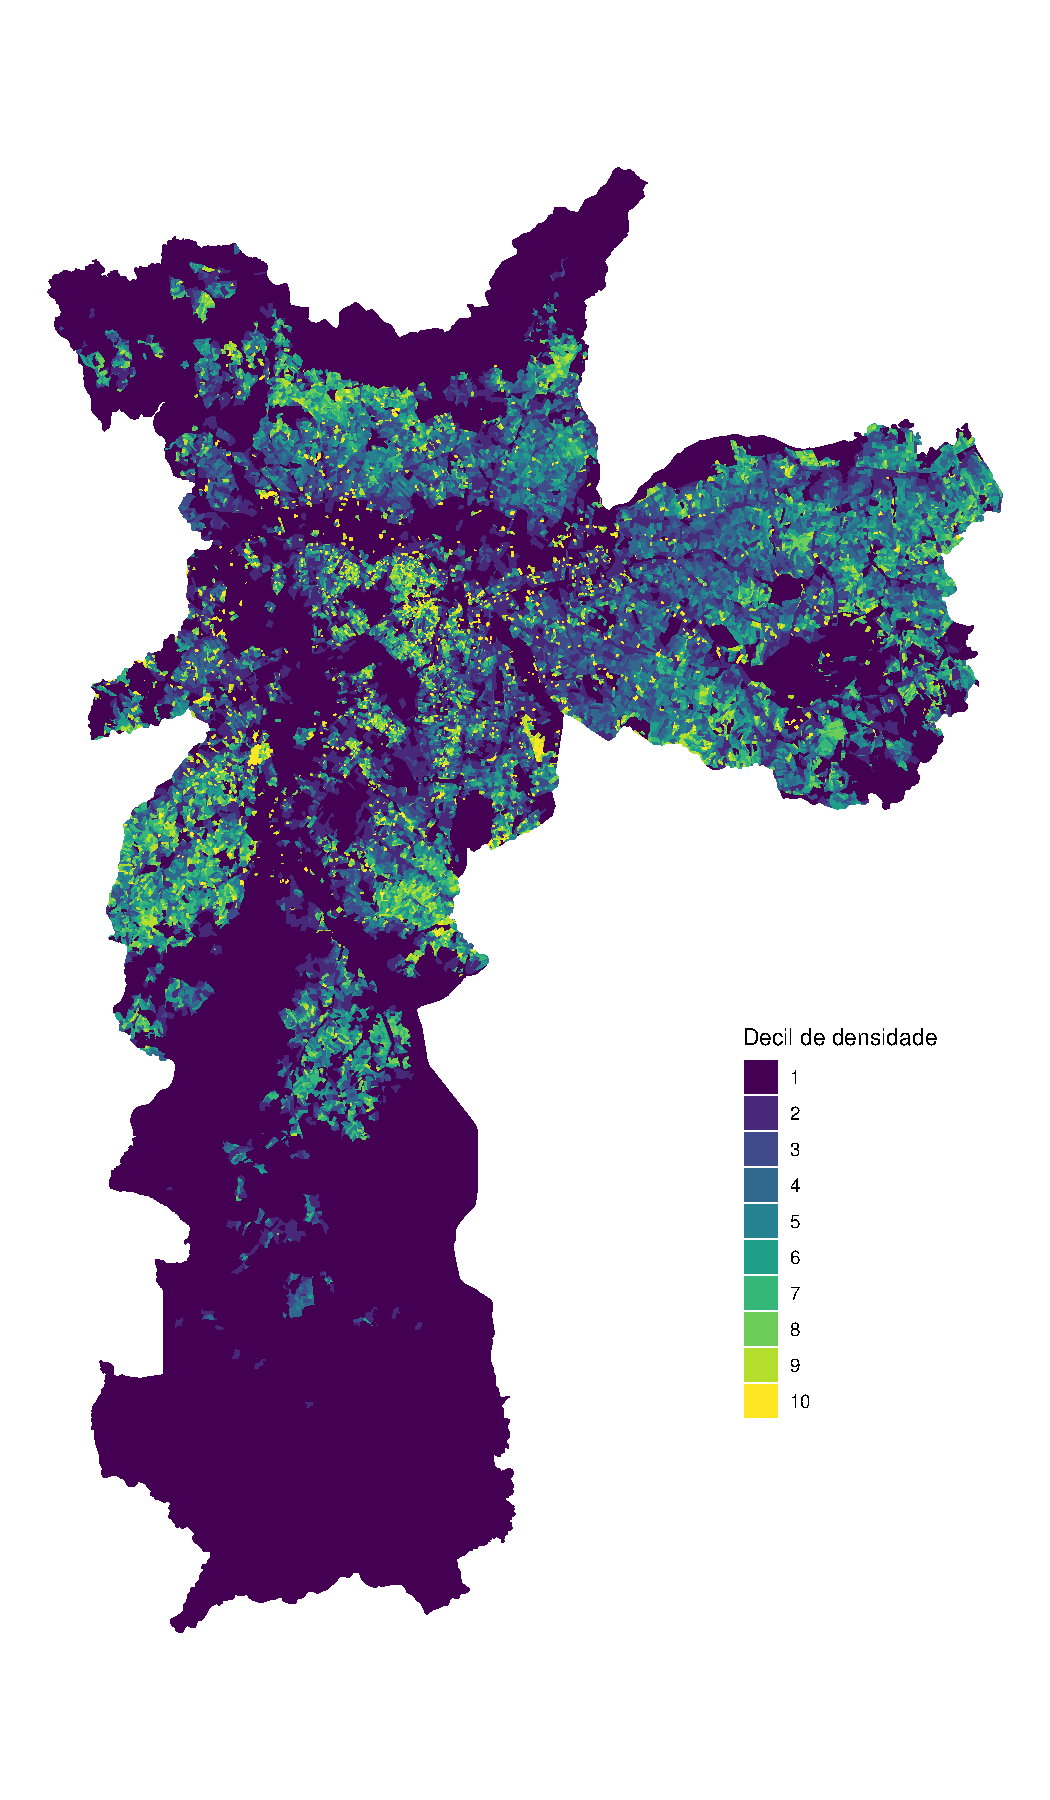
\includegraphics[height=.95\textheight]{imagens/mapa.pdf}
        \end{figure}

        \column{.6\textwidth}
        \begin{itemize}
            \item Dados preliminares do Censo de 2022
            \item Nível da observação: setor censitário
            \item 11.451.999 de habitantes e 4.996.529 de domicílios, dos quais 4.316.336 estão ocupados
        \end{itemize}
        \begin{figure}
            \centering
            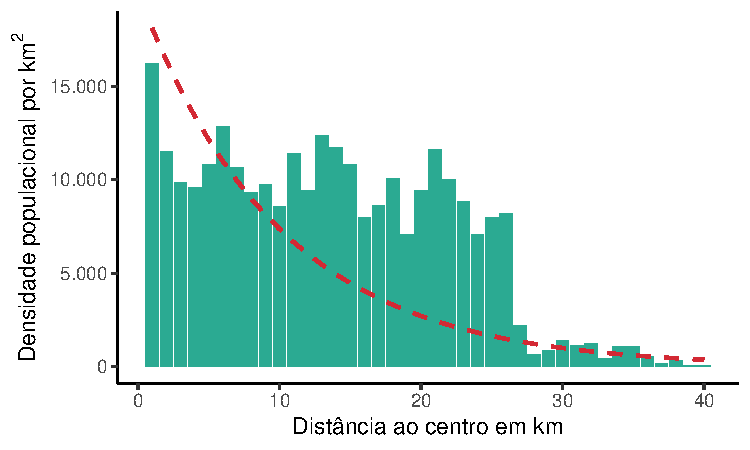
\includegraphics[width = .7\textwidth]{imagens/densidade_distcentro.pdf}
        \end{figure}
        
        
    
    \end{columns}
\end{frame}

\begin{frame}
    \frametitle{Dados do IPTU}
    \begin{itemize}
        \item Estoque (e não fluxo) imobiliário.
        \item Estão cadastrados 3.096.719 contribuintes, dos quais \textcolor{BrickRed}{2.641.635} são habitacionais
    \end{itemize}
    \begin{figure}
        \centering
        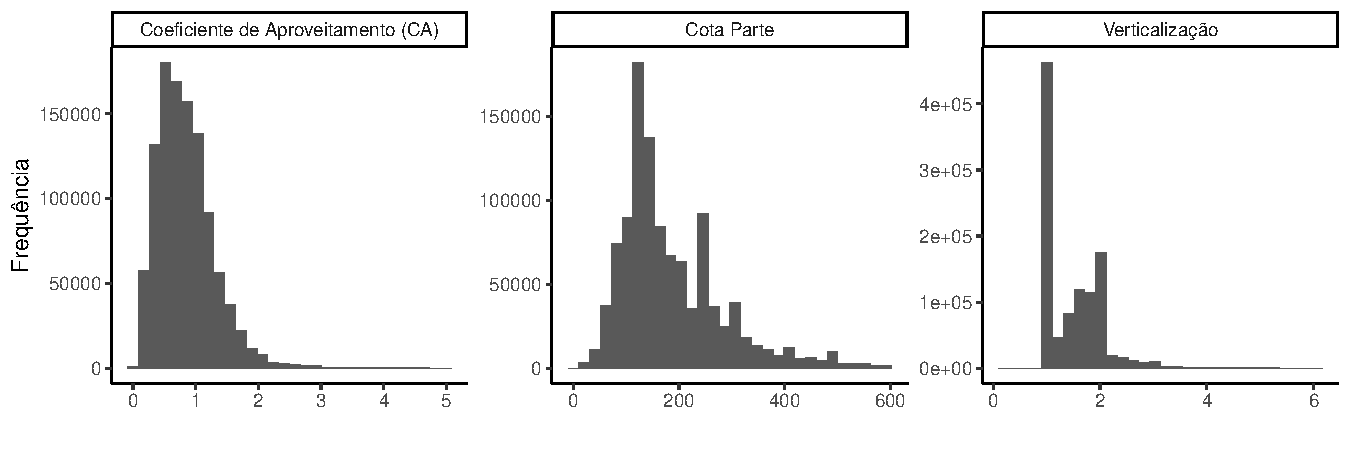
\includegraphics[width = .6\textwidth]{imagens/indicadores.pdf}
    \end{figure}
\end{frame}

\begin{frame}
    \frametitle{Dados do IPTU}
    \begin{figure}
        \centering
        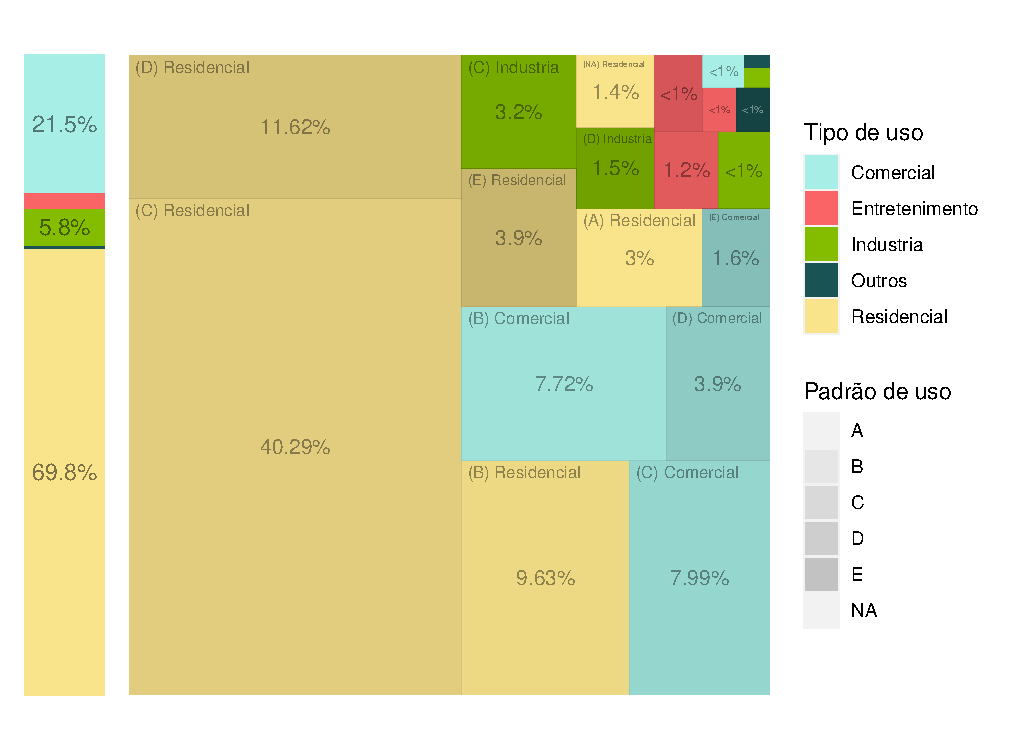
\includegraphics[height = .95\textheight]{imagens/tree_area_construida.pdf}
    \end{figure}
\end{frame}

\begin{frame}
    \frametitle{Cruzamento dos dados}
\end{frame}

\section{Análise}

\begin{frame}
    \frametitle{Construção do modelo empírico}
\end{frame}

\begin{frame}
    \frametitle{Resultados}
\end{frame}

\section{Conclusão}

\begin{frame}
    \frametitle{Resultados}
\end{frame}

% \section{teste2}
% \begin{frame}
% \frametitle{Columns}
% \begin{columns}
%     \column{0.5\textwidth}
%     Left column content.
%     \column{0.5\textwidth}
%     Right column content.
% \end{columns}
% \end{frame}


\end{document}
